%! Tex program = xelatex
\documentclass[UTF8]{ctexart}
% \documentclass{article}
\usepackage{fancyhdr}
\usepackage{extramarks}
\usepackage{amsmath}
\usepackage{amsthm}
\usepackage{amsfonts}
\usepackage{tikz}
\usepackage[plain]{algorithm}
\usepackage{algpseudocode}
\usepackage{pgfplots}
\usepackage{graphicx}
\usepackage{subfigure}
\usetikzlibrary{automata,positioning}

%
% Basic Document Settings
%

\topmargin=-0.45in
\evensidemargin=0in
\oddsidemargin=0in
\textwidth=6.5in
\textheight=9.0in
\headsep=0.25in

\linespread{1.1}

\pagestyle{fancy}
\lhead{\hmwkAuthorName}
\chead{\hmwkClass\ (\hmwkClassInstructor\ \hmwkClassTime): \hmwkTitle}
\rhead{\firstxmark}
\lfoot{\lastxmark}
\cfoot{\thepage}

\renewcommand\headrulewidth{0.4pt}
\renewcommand\footrulewidth{0.4pt}

\setlength\parindent{0pt}

%
% Create Problem Sections
%

\newcommand{\enterProblemHeader}[1]{
    \nobreak\extramarks{}{Assignment \arabic{#1} continued on next page\ldots}\nobreak{}
    \nobreak\extramarks{Assignment \arabic{#1} (continued)}{Assignment \arabic{#1} continued on next page\ldots}\nobreak{}
}

\newcommand{\exitProblemHeader}[1]{
    \nobreak\extramarks{Assignment \arabic{#1} (continued)}{Assignment \arabic{#1} continued on next page\ldots}\nobreak{}
    \stepcounter{#1}
    \nobreak\extramarks{Assignment \arabic{#1}}{}\nobreak{}
}

\setcounter{secnumdepth}{0}
\newcounter{partCounter}
\newcounter{homeworkProblemCounter}
\setcounter{homeworkProblemCounter}{1}
\nobreak\extramarks{Assignment \arabic{homeworkProblemCounter}}{}\nobreak{}

\newenvironment{homeworkProblem}{
    \section{Assignment \arabic{homeworkProblemCounter}}
    \setcounter{partCounter}{1}
    \enterProblemHeader{homeworkProblemCounter}
}{
    \exitProblemHeader{homeworkProblemCounter}
}

%
% Homework Details
%   - Title
%   - Due date
%   - Class
%   - Section/Time
%   - Instructor
%   - Author
%

\newcommand{\hmwkTitle}{第四次}
\newcommand{\hmwkDueDate}{2020年3月30日}
\newcommand{\hmwkClass}{流体力学导论作业}
\newcommand{\hmwkClassTime}{天文系}
\newcommand{\hmwkClassInstructor}{北京师范大学}
\newcommand{\hmwkAuthorName}{王正一 201711160128}

%
% Title Page
%

\title{
    \vspace{2in}
    \textmd{\textbf{\hmwkClass:\ \hmwkTitle}}\\
    % \normalsize\vspace{0.1in}\small{交\ 于\ \hmwkDueDate\ 8:00am }\\
    \vspace{0.1in}\large{\textit{\hmwkClassInstructor\hmwkClassTime}}
    \vspace{3in}
}

\author{\textbf{\hmwkAuthorName}}
\date{}

\renewcommand{\part}[1]{\textbf{\large Part \Alph{partCounter}}\stepcounter{partCounter}\\}
\renewcommand{\QQQ}[1]{\textbf{\large Question \Alph{partCounter}}\stepcounter{partCounter}\\}

%
% Various Helper Commands
%

% Useful for algorithms
\newcommand{\alg}[1]{\textsc{\bfseries \footnotesize #1}}

% For derivatives
\newcommand{\deriv}[1]{\frac{\mathrm{d}}{\mathrm{d}x} (#1)}
\newcommand{\derivt}[1]{\frac{\mathrm{d}}{\mathrm{d}t} (#1)}
\newcommand{\Derivt}[1]{\frac{\mathrm{D}}{\mathrm{D}t} (#1)}
\newcommand{\derivo}[2]{\frac{\mathrm{d} #1 }{\mathrm{d} #2}}
\newcommand{\derivp}[2]{\frac{\partial #1}{\partial #2}}
% For partial derivatives
\newcommand{\pderiv}[2]{\frac{\partial}{\partial #1} (#2)}

% Integral dx
\newcommand{\dx}{\mathrm{d}x}

% Alias for the Solution section header
\newcommand{\solution}{\textbf{\large Solution}}

% Probability commands: Expectation, Variance, Covariance, Bias
% \newommand{\E}{\mathrm{E}}
% \newcommand{\Var}{\mathrm{Var}}
% \newcommand{\Cov}{\mathrm{Cov}}
% \newcommand{\Bias}{\mathrm{Bias}}

\begin{document}

\maketitle

\pagebreak

\begin{homeworkProblem}
\QQQ{1}
    给定平面标量场 \(\phi\) . 设在M点上已知两个方向\(\vec{s_{1}}\) 和 \(\vec{s_{2}}\) , 
    的方向导数分别为 \(\frac{\partial \phi}{\partial \vec{s_{1}}}\) 
    和 \(\frac{\partial \phi}{\partial \vec{s_{2}}}\) 
    \[
      \bar{MP}=\derivp{\phi}{s_{2}}
      ,\bar{MK}=\derivp{\phi}{s_{1}}
    \]
    \[
      |\vec{s_{1}}|=|\vec{s_{2}}|=1
    \]

    \begin{figure}[h]
    \centering
    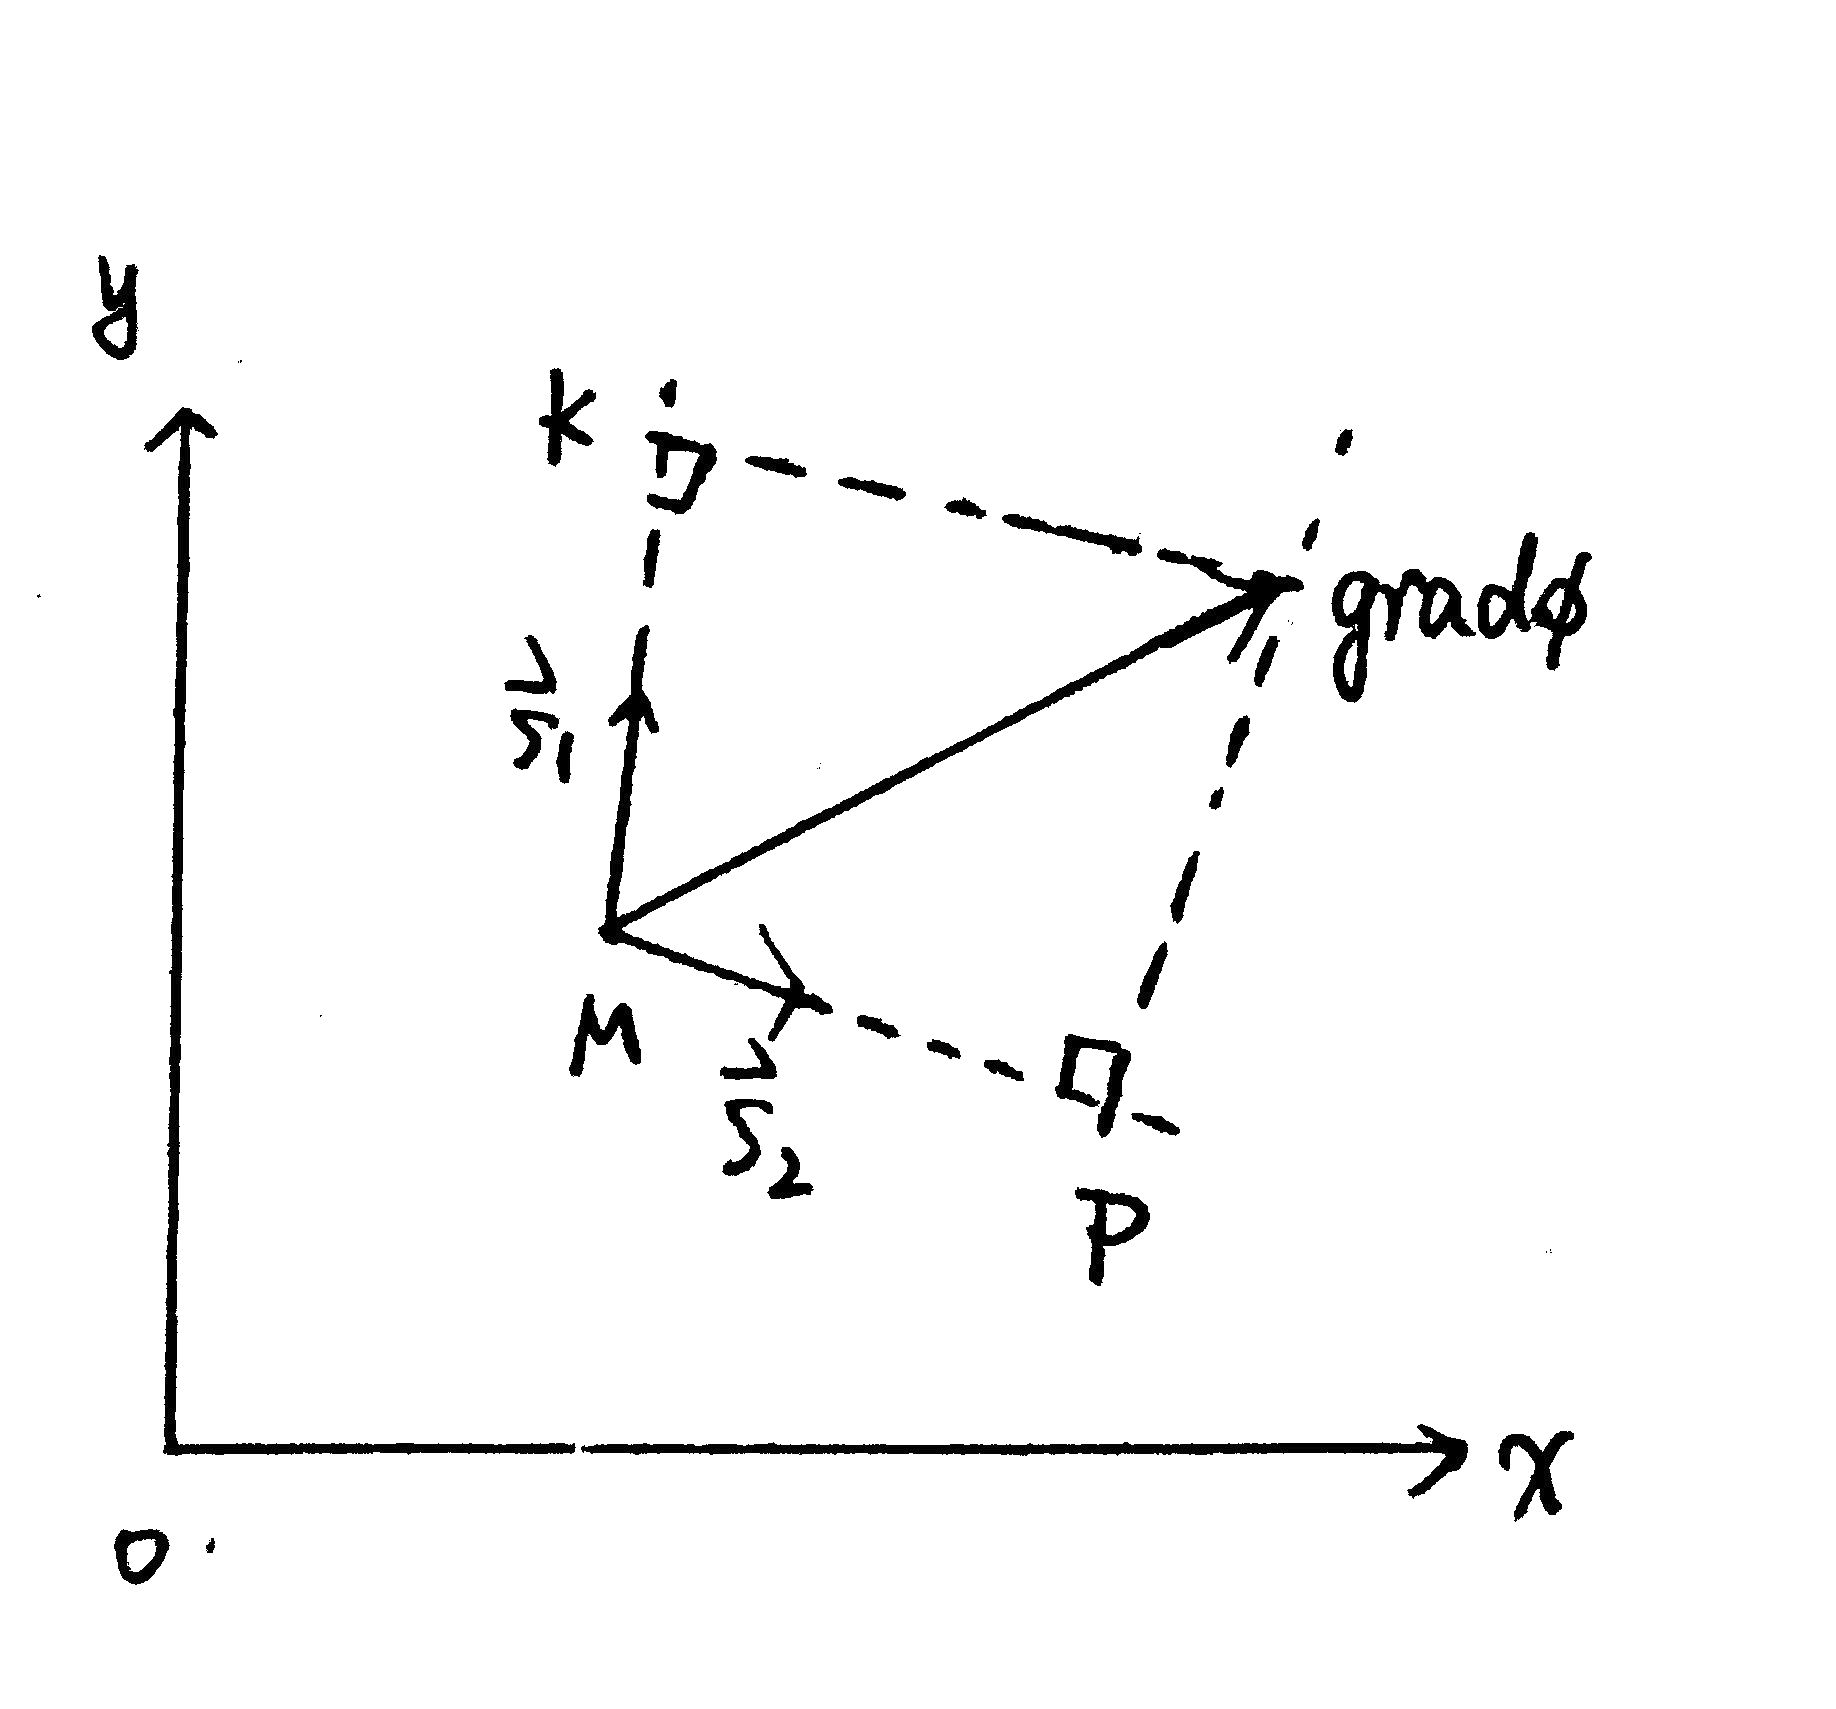
\includegraphics[width=12cm]{3}
    \caption{第一题图(手绘)}
    \end{figure}

   

\QQQ{2}
    利用散度\(\text{div}\) \(\vec{a}\) 的定义推导它在球坐标系中的表达式.

    \[
		\begin{aligned}
			\\
			&\nabla \cdot \vec{a} \cdot r^{2} \sin \theta d r d \theta d \phi 
			\\
			&= \frac{\partial }{\partial r} \left( r^{2} \sin \theta a_{r} \right) d r d \theta d \phi + \frac{\partial }{\partial \theta} \left( r \sin \theta a_{\theta} \right) d r d \theta d \phi + \frac{\partial }{\partial \phi} \left( r a_{\phi} \right) d r d \theta d \phi &
			\\
			&\nabla \cdot \vec{a} & 
			\\
			& = \frac{1}{r^{2} \sin \theta d r d \theta d \phi} \left[ \frac{\partial }{\partial r} \left( r^{2} \sin \theta a_{r} \right) d r d \theta d \phi + \frac{\partial }{\partial \theta} \left( r \sin \theta a_{\theta} \right) d r d \theta d \phi + \frac{\partial }{\partial \phi} \left( r a_{\phi} \right) d r d \theta d \phi \right] &
			\\
			&= \frac{1}{r^{2}} \frac{\partial}{\partial r}\left(r^{2} a_{r}\right)+\frac{1}{r \sin \theta} \frac{\partial}{\partial \theta}\left(\sin \theta a_{\theta}\right)+\frac{1}{r \sin \theta} \frac{\partial a_{\phi}}{\partial \phi}
		\end{aligned}
	\]
\QQQ{3}
	\(
	{\text{已知矢量}}\vec{a}{\text{在球坐标系中的三个分量分别为:}}
	a_{r} = \frac{2k \cos \theta}{r^{3}},a_{\theta} = \frac{k \sin \theta}{r^{3}} , a_{\phi}=0
	{\text{其中k为一常数。试验证矢量}}\vec{a}{\text{是否为位势矢量,若是则}} \varphi {\text{等于什么,并求矢
	量}} \vec{a} {\text{经过球面}}r = R {\text{的通量.}}\)
	
	\[
		\begin{aligned}
			&\frac{\partial \varphi}{\partial r}= \frac{2k \cos \theta}{r^{3}}
			\\
			&\frac{1}{r} \frac{\partial \varphi}{\partial \theta}= \frac{k \sin \theta}{r^{3}}
			\\
			&\frac{\partial \varphi}{\partial \phi}= 0
			\\
		\end{aligned}
	\]
	\text{若加以边界条件:}
	\[
		\begin{aligned}
			&\varphi |_{r \rightarrow \infty} = 0
			\\
			&\varphi = - \frac{k \cos \theta}{r^{2}}
			\\
		\end{aligned}
	\]
\end{homeworkProblem}

\pagebreak

\begin{homeworkProblem}
\QQQ{1}  
    一平板重为\( mg=1000N\) ,面积为\( A=0.16 m^{2}\) 。板下涂满油,沿与水平线成
    \( \theta = 20^{\circ} \) 的 斜 平 壁 下 滑 , 油 膜 厚 度 为\( h = 0.005 mm\)。 若 油 的 粘 度 为
    \( \mu = 0.007 pa \cdot s\),求板下滑的终端速度\(V\)。
    \( \\ \)
    平板受力平衡时:
    \[
        \begin{aligned}
            &\mu \frac{\partial v}{\partial y} A = mg \sin \theta
            \\
            &\frac{\partial v}{\partial y} \approx \frac{V}{h}
            \\
            &V = \frac{mgh \sin \theta}{\mu A} \approx 1.527 m/s
        \end{aligned}
\]
\QQQ{2}
        
    旋转圆筒粘度计的内容的直径为\(d=30cm\),高为\(h=30cm\),外筒与内筒的间隙为 \(\delta = 0.2cm \),间隙中充满被测流体。
    外筒做匀速旋转,角速度为\(\omega = 15 rad/s \)。测出作用在精致内筒的力矩为\(M=8.5N \cdot m\),
    忽略筒底部的阻力,求被测流体的粘度\(\mu \)。

    \[
        \begin{aligned}
            &\mu \frac{d V}{d r} S = \frac{M}{d/2}
            \\
            &\mu \frac{d V}{d r} \cdot \pi d h = \mu \frac{\omega d}{2 \delta}  = \frac{M}{d/2}
            \\
            &\mu = \frac{4M \delt}{\pi \omega d^{3}h} \approx 89.074 Pa \cdot s
            \\
        \end{aligned}
    \]

\QQQ{3}
    根据声速的定义(微小扰动在流体中的传播速度)的定义推导其定量计算的公式\(c_{s}=\sqrt{dp/d \rho}=\sqrt{k/ \rho}\),
        其中\(K\)为流体的体积模量。
    \begin{figure}[h]
    \centering
    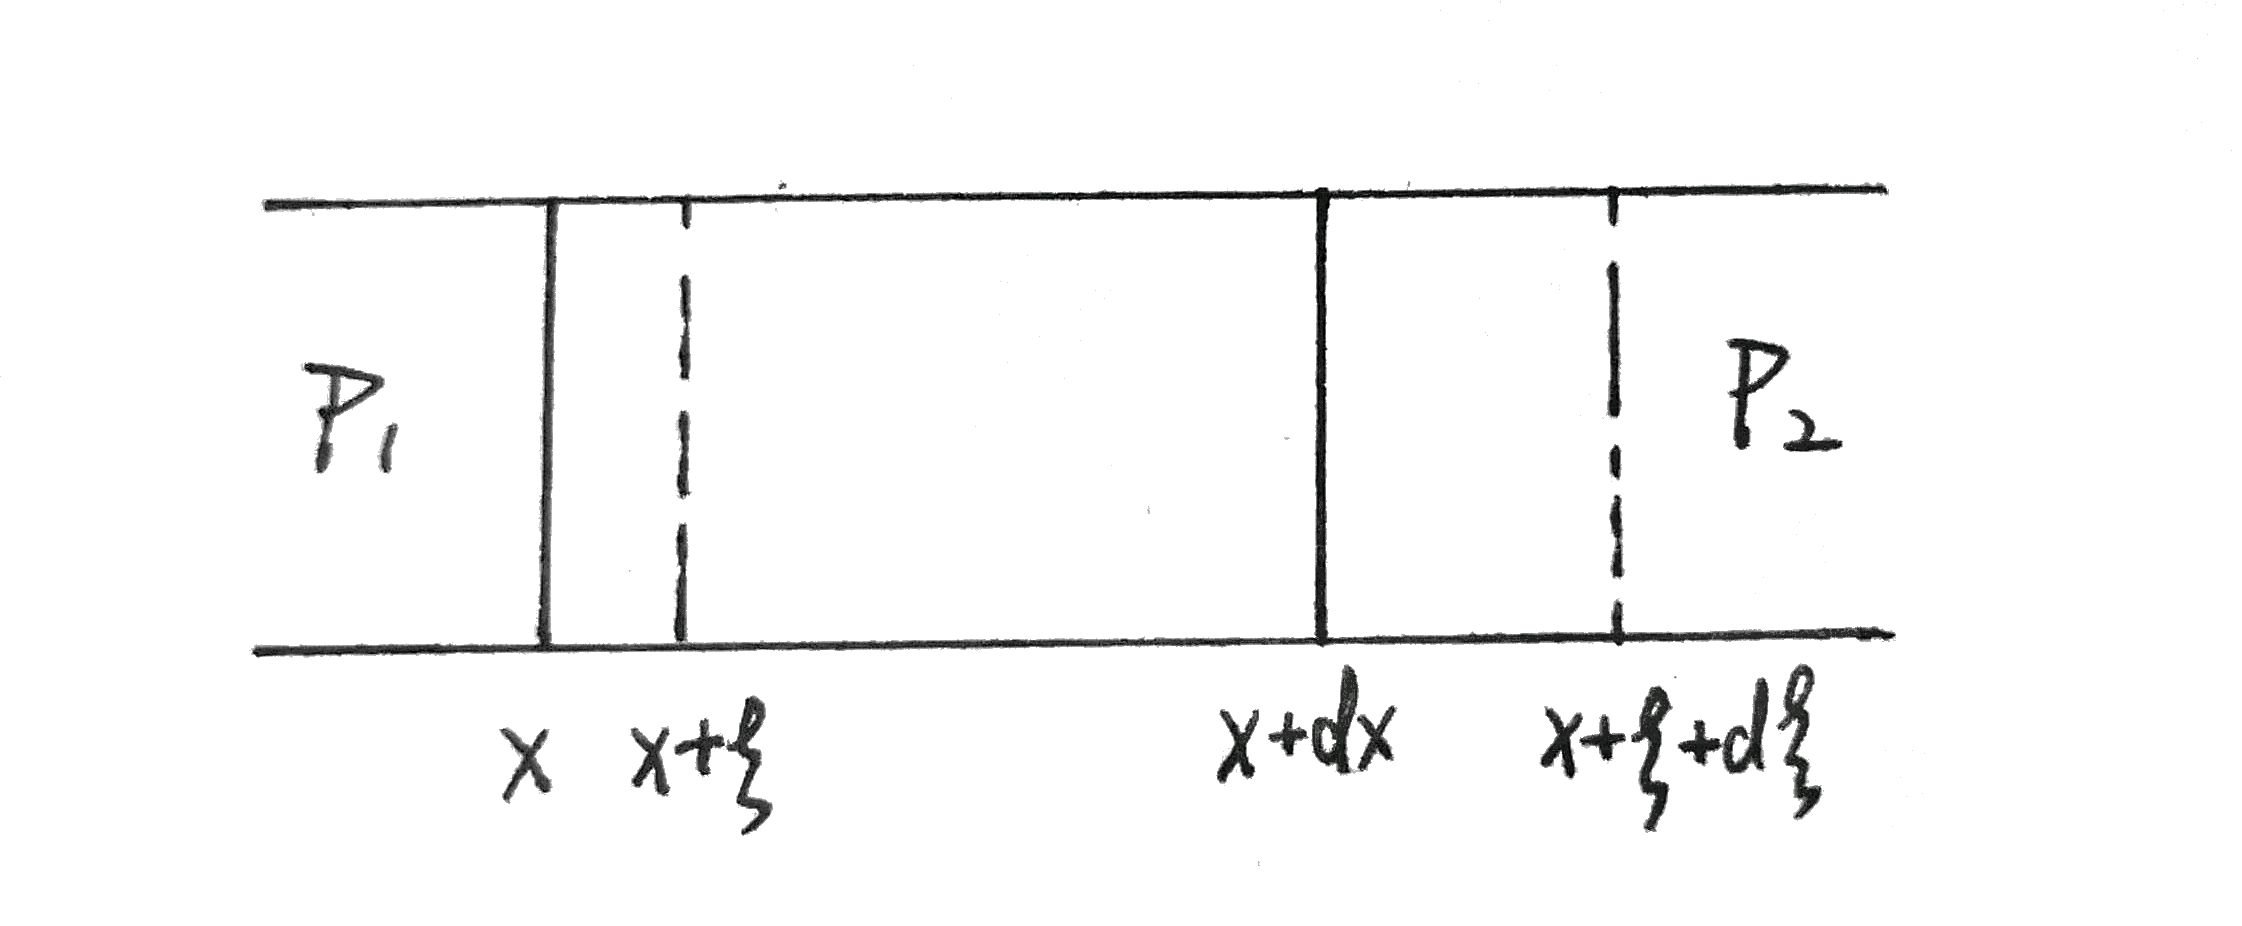
\includegraphics[width=14cm]{2}
    \caption{第三题图(手绘)}
    \end{figure}
    \[
        \begin{split}
            &\frac{\Delta V}{V} = \frac{\Delta \xi}{ \Delta x } = \frac{\partial \xi}{\partial x}
            \\
            &d p = \frac{d p }{d \rho} d \rho =-\frac{dp}{d \rho} \rho \frac{dv}{v}=-\frac{dp}{d\rho}\rho \frac{\partial \xi}{\partial x}
            \\
            &p_{1} =p_{0}+\left(dp \right)_{x}=p_{0}-\frac{dp}{d \rho } \rho \frac{\partial \xi}{\partial x}|_{x}
            \\
            &p_{2} =p_{0}+\left(dp \right)_{x+dx}=p_{0}-\frac{dp}{d\rho}\rho \frac{\partial \xi}{\partial x}|_{x+dx}
            \\
        \end{split}
    \]
      \leftline{牛顿第二定律:}
    \[
        \begin{split}
            \\
            &\left(p_{1}-p_{2}\right)S =\rho S \frac{\partial^{2} \xi}{\partial t^{2}}dx
            \\
            &p_{1}-p_{2} = \ \frac{dp}{d\rho} \rho \left(\frac{\partial \xi}{\partial x}|_{x+dx} - \frac{\partial \xi}{\partial x}|_{x}\right) = \frac{dp}{d\rho}\rho\frac{\partial^{2} \xi}{\partial x^{2}}dx = \rho \frac{\partial^{2} \xi} {\partial t^{2}}dx
            \\
        \end{split}
    \]
      \leftline{即:}
    \[
        \begin{split}
            &\frac{ \partial^{2} \xi }{ \partial t^{2} } - \frac{ d p }{d \rho } \frac{ \partial^{2} \xi}{ \partial x^{2} } =0
            \\
            &K=-\frac{dp}{dv/v}=\frac{dp}{\frac{d\left(1/\rho\right)}{1/\rho}}=\rho \frac{dp}{d\rho}
            \\
        \end{split}
    \]
      \leftline{所以:}
    \[
        \begin{split}
            &c_{s}=\sqrt{\frac{dp}{d\rho}}=\sqrt{\frac{K}{\rho}}
            \\
        \end{split}
    \]

\end{homeworkProblem}
\pagebreak
\begin{homeworkProblem}
\QQQ{1}
  设\(u=x+t  ,  v=-y+t ,\omega = 0 \),求通过\(x=-1  , y=-1\)的流线及\(t=0\)时通过\(x=-1  ,  y=-1\)的迹线。
  \\
  流线方程:
  \[
    \frac{dx}{x+t} = \frac{dy}{-y+t}
  \]
  积分后得:
  \[
    \left(x+t \right)\left(-y +t \right) = C
  \]
  而\(t=0\ , x=-1  , y=-1 ,\text{因此} C=1\),所以流线方程是:
  \[
    xy=1
  \]
  迹线方程:
  \[
    &\derivo{x}{t}=x+t,
    \
    &\derivo{y}{t}=-y+t
    \
  \]
  解得:
  \[
    &x=C_{1}e^{t}-t-1,
    \
    &y=C_{2}e^{-t}+t-1
    \
  \]
  而\(t=0\ , x=-1  , y=-1 ,\text{因此} C_{1}=C_{2}=0\),所以迹线方程是:
  \[
    x+y=-2
  \]
\QQQ{2}
  设\(u=\frac{cx}{x^{2}+y^{2}}  , v={cy}{x^{2}+y^{2}}  , \omega = 0 \),求流线方程并画图。
  \\
  流线方程:
  \[
    \frac{dx}{u} = \frac{dy}{v}
  \]
  即为:
  \[
    \frac{dx}{x} = \frac{dy}{y}
  \]
  解得:
  \[
    y=kx  \left( k \text{是任意常数} \right)
  \]
  流线图:
  \[
  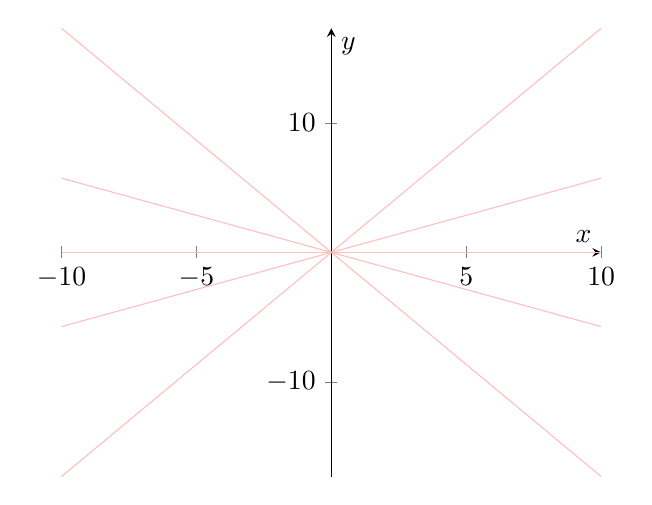
\begin{tikzpicture}
  \begin{axis}[
      axis lines = center,
      xlabel = {$x$},
      ylabel = {$y$},
  ]
  %Below the red parabola is defined
  \addplot [
      domain=-10:10, 
      samples=100, 
      color=pink,
  ]
  {0};
  \addplot [
      domain=-10:10, 
      samples=100, 
      color=pink,
  ]
  {1.73205*x};
  \addplot [
      domain=-10:10, 
      samples=100, 
      color=pink,
  ]
  {0.5735*x};
  \addplot [
      domain=-10:10, 
      samples=100, 
      color=pink,
  ]
  {-1.73205*x};
  \addplot [
      domain=-10:10, 
      samples=100, 
      color=pink,
  ]
  {-0.5735*x}; 


  \end{axis}
  \end{tikzpicture}
  \]
  
\QQQ{3}
  设平面不定常流动的速度分布为\(u=x\left( 1+2t \right),v=y\),求通过点\(\left(1,2 \right)\)流线方程并画\(t_{1}=0,t_{2}=2\)时刻过点\(\left(1,2\right)\)的流线图。
  \\
  流线方程:
  \[
    \frac{dx}{x\left( 1+2t \right)} = \frac{dy}{y}
  \]
  积分得:
  \[
    \frac{1}{1+2t} \ln x = \ln Cy
  \]
  而\( x=1 , y=2 ,\text{因此} C=\frac{1}{2}\),所以:
  \[
    x=\left( \frac{y}{2} \right)^{1+2t}
  \]
  流线图:
  \[
  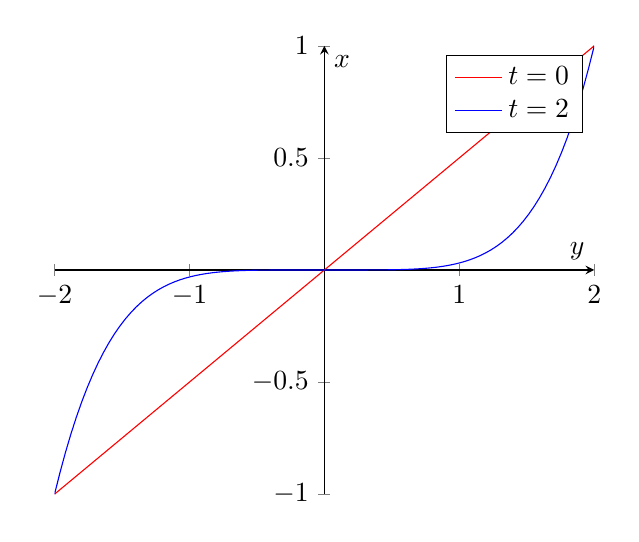
\begin{tikzpicture}
  \begin{axis}[
      axis lines = center,
      xlabel = {$y$},
      ylabel = {$x$},
  ]
  %Below the red parabola is defined
  \addplot [
      domain=-2:2, 
      samples=100, 
      color=red,
  ]
  {x/2};
  \addlegendentry{$t=0$}
  %Here the blue parabloa is defined
  \addplot [
      domain=-2:2, 
      samples=100, 
      color=blue,
      ]
      {(x/2)^5};
  \addlegendentry{$t=2$}

  \end{axis}
  \end{tikzpicture}
  \]

\end{homeworkProblem}


\pagebreak
\begin{homeworkProblem}
\QQQ{1}
  已知流场的速度分布为\(u=4x^{3},v=-10x^{2}y,\omega = 2t\),试问(求):
  \\
  1.该流场属于几维流动?
  \\
  流场在三个方向都有速度分量,所以是三维流动、
  \\
  2.\(t=1\)时点\(\left( 2,1,3 \right)\)处的加速度:
  \\
  \[
    \begin{aligned}
      &\vec{a}= \frac{D\vec{V}}{Dt}=\derivp{\vec{V}}{t}+\vec{V} \cdot \nabla \vec{V}
      \\
      &a_{x}=\derivp{u}{t} + u \derivp{u}{x}+ v \derivp{u}{y}+ \omega \derivp{u}{z}=48x^{5}
      \\
      &a_{y}=\derivp{v}{t} + u \derivp{v}{x}+ v \derivp{v}{y}+ \omega \derivp{v}{z}=20x^{4}y
      \\
      &a_{z}=\derivp{\omega}{t} + u \derivp{\omega}{x}+ v \derivp{\omega}{y}+ \omega \derivp{\omega}{z}=2
    \end{aligned}
  \]
  所以加速度是:
  \[
    \vec{a}=\left(48x^{5} ,20x^{4}y,2 \right)
  \]
\QQQ{2}
  \[
    \begin{aligned}
      &\delta \vec{r} = \vec{r} - \vec{r_{0}}
      \\
      &\derivt{\delta \vec{r}} = \delta \vec{v} = \delta \derivt{\vec{r}}
    \end{aligned}
  \]
  即 \(\delta\)和\(\derivt{ }\)可以互换。
  \\
  因此:
  \[
    \Derivet{\delta \vec{r}} = \delta \vec{v} + \delta \vec{r} \cdot \nabla \vec{v}
  \]
\QQQ{3}
  1.求\(\oint \vec{V} \cdot d \vec{l} \)
  斯托克斯公式:
  \[
    \oint \vec{V} \cdot d \vec{l} = \iint_{S} \nabla \times \vec{V} \cdot d \vec{S}=0
  \]


  2.求\(\nabla \times \vec{V}\)
  \[
    \begin{aligned}
      \nabla \times \vec{V}&=\left(\frac{1}{r} \frac{\partial v_{z}}{\partial \phi}-\frac{\partial v_{\phi}}{\partial z}\right) \boldsymbol{e_{r}}+\left(\frac{\partial v_{r}}{\partial z}-\frac{\partial v_{z}}{\partial r}\right) \boldsymbol{e_{\phi}} + \left[\frac{1}{r} \frac{\partial}{\partial r}\left(r v_{\phi}\right)-\frac{1}{r} \frac{\partial v_{r}}{\partial \phi}\right] \boldsymbol{e_{z}}
      \\
      \\
      &=\frac{1}{r} \derivp{rv_{\phi}}{r}\boldsymbol{e_{z}}
      \\
      &=\boldsymbol{0}
    \end{aligned}
  \]

\end{homeworkProblem}
\end{document}
